\documentclass[12pt]{article}
\usepackage[left=3cm, top=3cm, right=3cm, bottom=3cm]{geometry}
\usepackage[utf8]{inputenc}      % accents dans le source
\usepackage[T1]{fontenc}
\usepackage[french]{babel}
\usepackage{graphicx}
\usepackage{graphics}
\usepackage{amsmath}
\usepackage{tikz}
\usepackage{xcolor} 
\usepackage{mathtools}
\usepackage{parskip}
\usepackage{subcaption}
\usepackage[export]{adjustbox}
\usepackage{chemist}

\title{\textbf{TP1 Chimie des Solutions} \\ Dosage colorimétrique de l’aspirine dans un comprimé}
\author{MENARD Alexandre \\ VIEILLEDENT Florent}

\begin{document}
\maketitle

\section*{Introduction}

Dans ce travail pratique, on déterminera la masse d'acide acétylsalicylique dans un comprimé d'aspirine grâce à un titrage par de la soude. 
On commencera par étalonner notre solution de soude par dosage pH-métrique et dosage colorimétrique avec de l'acide oxalique. Puis on effectuera les même dosages mais avec de l'acide acétylsalicylique et notre soude étalonnée. 
\newpage

\section{Étalonnage de la solution de soude}

Le but de cette première expérience est de déterminer précisément la concentration d'une solution pour l'utiliser par la suite pour titrer une autre solution. On dose notre solution par de l'acide oxalique en utilisant du phénolphtaléine comme colorant pour la colorimétrie. On effectue un dosage pH-métrique en même temps. 

	\subsection{Montage expérimental}
	
\begin{figure}[!h]
	\begin{center}
\includegraphics[scale=0.2]{Schéma_Titrage1.png}
\label{Schéma_Titrage1}
\caption{Schéma du montage expérimental du titrage de la soude par l'acide oxalique}
\end{center}
\end{figure}

On pèse $m_{oxa}=60\pm 10$ mg d'acide oxalique, qu'on dissout dans une fiole jaugée de $V_{soln}=50.00\pm 0.06$ mL. On introduit la solution de soude de concentration inconnue dans une burette de $25$ mL graduée tous les millilitres. \textbf{Question 3:} on s'assure de bien laver la burette avec de la soude, pour que la valeur du volume de soude soit précise. On prélève $V_{oxa}=20.00\pm 0.03$ mL avec une pipette jaugée qu'on introduit dans un bécher de $50$ mL préalablement lavé. \textbf{Question 4:} le bécher n'a pas besoin d'être séché car c'est le nombre de mole d'acide oxalique qui est important. On installe dans le bécher les électrodes du pH-mètre qu'on a d'abord étalonné. On introduit aussi un barreau aimanté et quelques gouttes de phénolphtaléine. On réalise le titrage pH-métrique en notant la valeur du pH pour différentes valeurs de volume de soude versé. 
	
\newpage	
	\subsection{Résultat}
On trace la courbe du pH en fonction du volume de soude versé.
\begin{figure}[h!]
	\begin{center}
		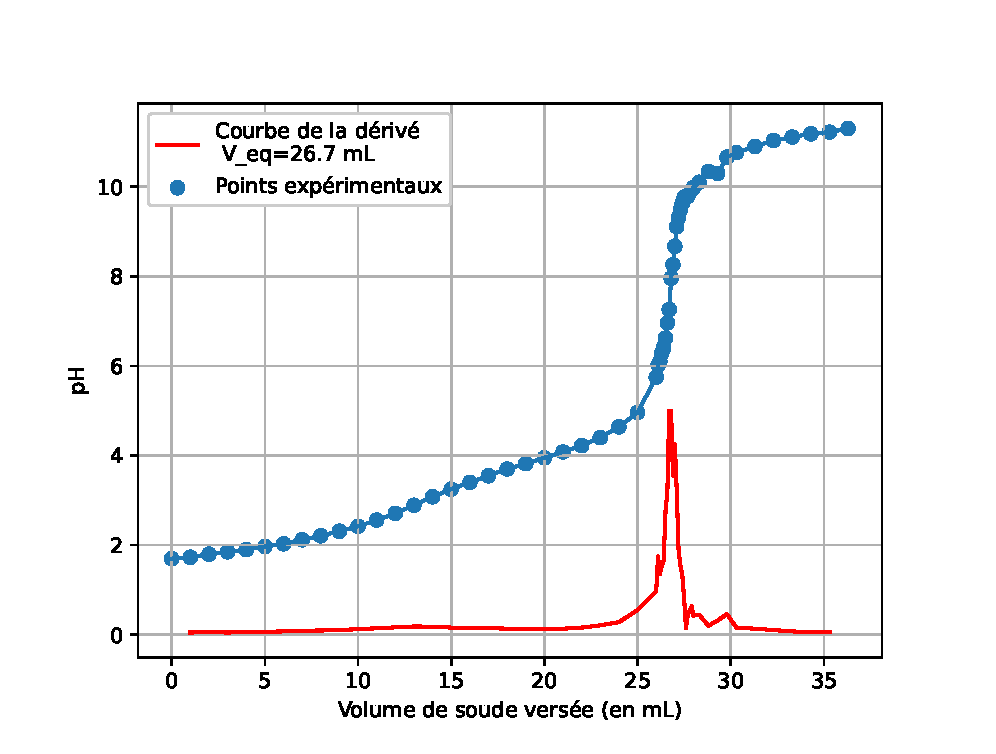
\includegraphics[scale=0.7]{Titrage_1.eps}
		\caption{Courbe du pH en fonction du volume de soude versé. On trace aussi la valeur de la dérivée en chaque point.}
		\label{Titrage_soude}
	\end{center}
\end{figure}	
	
	\subsection{Traitement des résultats}
	
La réaction entre l'acide oxalique et la soude est :
\begin{equation}
H_2C_2O_4+ 2 HO^- \longrightarrow C_2O_4^{2-} + H_2O
\end{equation}
D'après cette équation on a à l'équivalence : $n_{oxa}=\frac{n_{soude}}{2}$. On utilise la méthode de la dérivée pour trouver le volume à l'équivalence (voire graphique (\ref{Titrage_soude})). On trouve que le volume pour lequel la dérivée est la plus élevée est $26.7$ mL. On a donc $V_{eq}=26.7\pm 0.1 $ mL. \textbf{Question 1:} on cherche maintenant la valeur de la concentration de la solution de soude :
	\begin{align*}
C_{soude}V_{eq}=2C_{oxa}V_{oxa}& \Longrightarrow C_{soude} = \frac{2 m_{oxa} V_{oxa}}{V_{eq} M_{oxa} V_{soln}} \\
& \Longrightarrow C_{soude} = \frac{2*60*10^{-3}*20}{26.7*10^{-3}*126*50}\\ & \Longrightarrow C_{soude} =  0.0143 mol.L^{-1}		
	\end{align*}
	
On calcule l'incertitude relative
\begin{align*}
\frac{\Delta C_{soude}}{C_{soude}}&=\frac{\Delta m_{oxa}}{ m_{oxa}} +\frac{\Delta V_{oxa}}{ V_{oxa}} + \frac{\Delta V_{eq}}{V_{eq}} + \frac{\Delta V_{soln}}{V_{soln}} \\
\frac{\Delta C_{soude}}{C_{soude}}&= \frac{10}{60} + \frac{0,03}{20,00} + \frac{0,1}{26,7} + \frac{0,06}{50,00} \\
\frac{\Delta C_{soude}}{C_{soude}}&= 0.17 
\end{align*}

On calcule donc $\Delta C_{soude}=0.17*0.0143 = 0.0024$ mol/L. On a donc finalement $C_{soude}=0.014\pm 0.003$ mol/L.

	\subsection{Conclusion}
	
La valeur attendue pour la concentration était proche de $0.02$ mol/L. Nous trouvons une valeur inférieur avec un écart relatif de 30\%. C'est un écart significatif. Néanmoins nous avons une grande incertitude sur notre valeur, notamment à cause de l'incertitude sur la masse d'acide pesée. Effectivement, la balance de précision ne possédait pas de portes pour empêcher les courants d'airs, ce qui rend les mesures imprécises. Il faudrait refaire les manipulations en ayant une incertitude plus petites sur la masse pesée. 	
	
\section{Dosage de l'acide acétylsalicylique}
Le but de cette expérience est de déterminer le pourcentage massique d'acide acétylsalicylique dans un comprimé d'aspirine. Nous allons pour cela utiliser un titrage pH-métrique et colorimétrique. 

	\subsection{Montage expérimental}
\begin{figure}[h!]
	\begin{center}
		\includegraphics[scale=0.18]{Schéma_Titrage2.png}
		\label{Schéma_Titrage2}
		\caption{Schéma du montage expérimental du titrage de l'acide acétylsalicylique par de la soude}
	\end{center}
\end{figure}
On pèse le comprimé d'aspirine $m_{comprime}=490\pm 10$ mg. On réduit en poudre le comprimé et on le dissout dans une fiole jaugée de $V_{sola}=250,0\pm 0.2$ mL. Après avoir filtré notre solution, on en prélève $V_{asp}=20.00\pm 0.03$ mL qu'on introduit dans un bécher préalablement rincé. On lave une burette de $25$ mL avec notre solution de soude de concentration $C_{soude}=0.014\pm 0.003$ mol/L puis on introduit la solution de soude dedans. La burette est graduée tous les millilitres. On plonge les électrodes du pH-mètre dans le bécher et on introduit en même temps un barreau aimanté et du phénolphtaléine. On réalise ensuite le titrage en versant graduellement de la soude et en notant le pH de la solution. 

\newpage
	\subsection{Résultat}
On trace la courbe du pH en fonction du volume de soude versé. 
\begin{figure}[h!]
	\begin{center}
		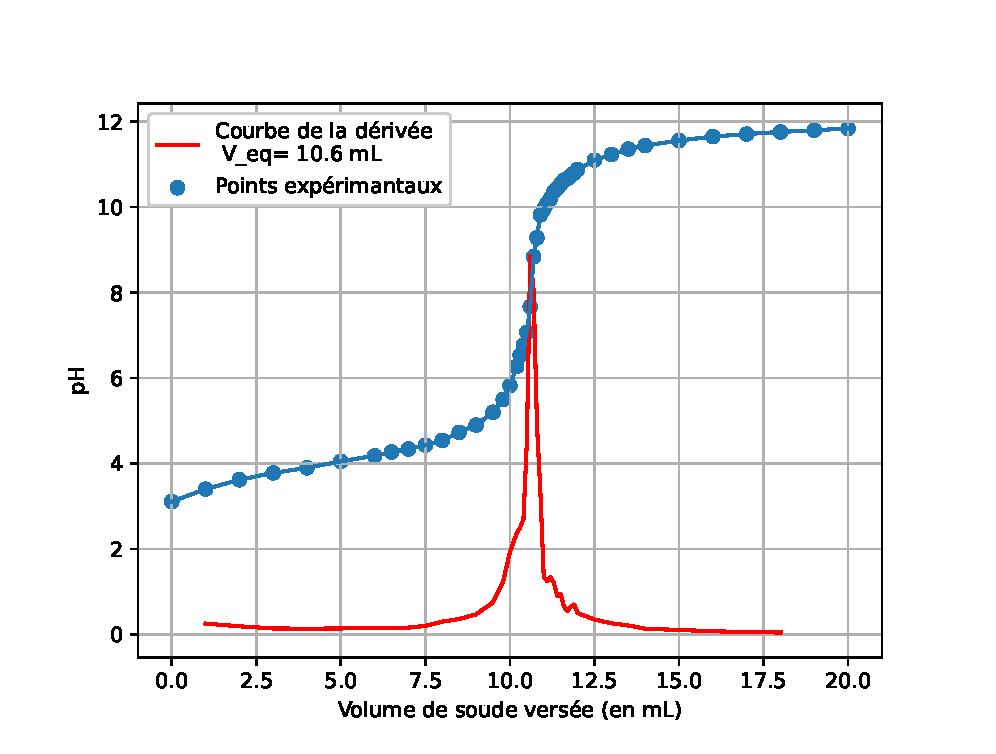
\includegraphics[scale=0.6]{Titrage_2.eps}
		\label{Titrage2}
		\caption{Courbe du pH en fonction du volume de soude versée. On trace aussi en rouge la valeur de la dérivée en chaque point.}
	\end{center}
\end{figure}

\newpage
	\subsection{Traitement des résultats}
On utilise la méthode de la dérivée pour obtenir le volume à l'équivalence. On obtient $V_{eq,soude}=10.6\pm 0.1$ mL.

\textbf{Question 6 :} On note $AH$ l'acide acétylsalicylique et $A^-$ sa base conjuguée (voire figure \ref{base} ). La réaction entre l'acide acétylsalicylique est alors:
\begin{equation}
AH + HO^- \longrightarrow A^- + H_2O
\label{Acidebase}
\end{equation}

\textbf{Question 5 :}	
\begin{figure}[h!]
	\begin{center}
		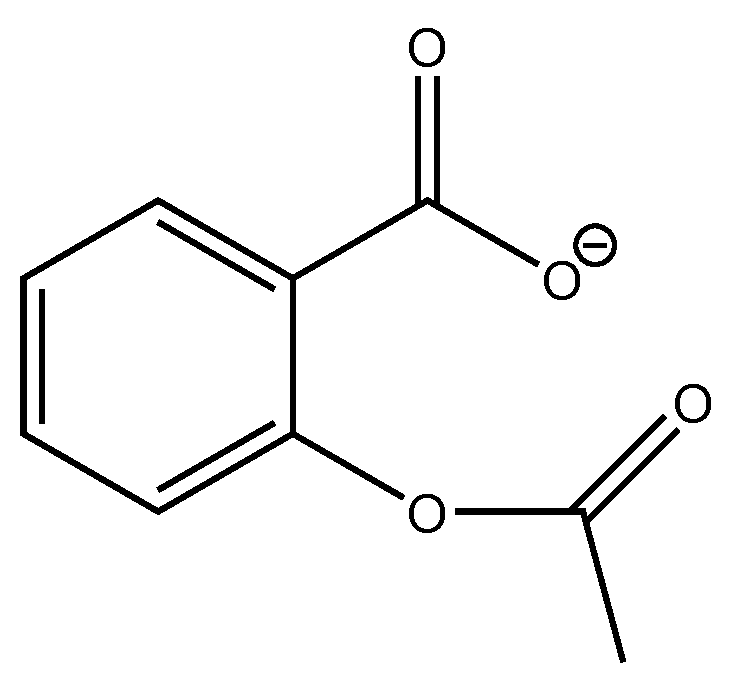
\includegraphics[scale=0.3]{base_aspirine.eps}
		\caption{Formule développée de la base conjuguée de l'acide acétylsalicylique}	
		\label{base}
	\end{center}
\end{figure}	

\textbf{Question 7 :}D'après l'équation (\ref{Acidebase}), on a la relation à l'équivalence : $n_{asp}=n_{soude}$. \textbf{Question 8 :} 
\begin{align*}
C_{asp}&=\frac{C_{soudes}V_{eq,soude}}{V_{asp}} \\
C_{asp}&=\frac{1.4*10.6}{20} \\
C_{asp}&=0.00742 mol.L^{-1}
\end{align*}

\textbf{Question 9 :} On calcule maintenant l'incertitude relative. 
\begin{align*}
\frac{\Delta C_{asp}}{C_{asp}}&=\frac{\Delta C_{soude}}{C_{soude}}+\frac{\Delta V_{eq,soude}}{V_{eq,soude}} + \frac{\Delta V_{asp}}{V_{asp}}\\
\frac{\Delta C_{asp}}{C_{asp}}&= 0.17 + \frac{0.1}{10.6} +\frac{0.2}{250} \\
\frac{\Delta C_{asp}}{C_{asp}}&= 0.18 
\end{align*}
On calcule $\Delta C_{asp}=0.18 * 0.00742 = 0.0013$ mol/L. Donc $C_{asp}=0.007 \pm 0.2$ mol/L. 
\textbf{Question 10 :} On a la relation : $C_m=C_{asp}+M_{asp}=0.007*180=1.26$ g/L. De plus $\frac{\Delta C_m}{C_m}=\frac{\Delta C_{asp}}{C_{asp}}=0.18$. Donc $\Delta C_m=1.26*0.18=0.23$ g/L. Donc $C_m=1.3\pm 0.3$ g/L. 

\textbf{Question 11 :} on obtient $ m_{asp}=C_m * V_{sola}=
1.3*250=325$ mg. L'incertitude est $\Delta m_{asp}=m_{asp}(\frac{\Delta C_m}{C_m}+ \frac{\Delta V_{sola}}{V_{sola}})=325(0.18+\frac{0.003}{20})=59$ mg. On a donc $m_{asp}=0.33\pm 0.06$ g. \\
\textbf{Question 12}: le pourcentage massique est donc $p=\frac{325}{500}= 65\%$. Son incertitude est $\Delta p= p(\frac{\Delta m_{asp}}{m_{asp}}+ \frac{\Delta m_{comprime}}{m_{comprime}})=0.65(\frac{59}{325}+\frac{10}{490})=13\%$. \\
Le pourcentage massique est donc finalement $p=0.7\pm 0.2$.
	
	\subsection{Conclusion}
\textbf{Question 13 :} Le pourcentage massique théorique est 100 \%. Même avec des incertitudes relatives importantes  on ne retrouve pas ce résultat. L'écart relatif entre le valeur théorique est de 30\% , ce qui est significatif et n'est pas expliqué par les incertitudes. Cela peut être causé par notre incertitude sur la concentration de la solution de soude. Il faudrait refaire l'expérience avec une valeur plus précise de cette concentration pour pouvoir conclure. 

\end{document}